\section{STEM}

\subsection{STEM (Scanning transmission electron microscopy)}

STEM-Mikroskopie unterscheidet sich zur CTEM-Mikroskopie maßgeblich im Abbildungsmechanismus, während bei CTEM wie zuvor beschrieben eine Parallele Beleuchtung verwendet wird, die ein großen Bereich auf der Probe durchleuchtet, wird beim STEM ein Konvergenter Elektronenstrahl verwendet der nur eine fokussierten Prunkt im Objekt durchleuchtet. Dieser wird mit Hilfe von Ablenkmagneten über die Probe gerastert, um eine Aufnahme zu erstellen. Dieses Verfahren bietet einige Vorteile, wie eine hohe Auflösung, aber auch die Möglichkeit von einer Ortsaufgelösten Spektroskopie. Dabei können verfahren verwendet werden wie EELS (Electron Energy Loss Spectroscopy) oder EDX (Energy Dispersive X-ray). Außerdem kann ein Elementarer Z- Kontrast durch HAADF gemessen werden und ortsaufgelöst dargestellt werden.

\subsection{JEOL JEM-ARM300F2}
In diesem Versuchsteil wurde das „JEOL JEM-ARM300F2 STEM“ verwendet, dieses Mikroskop arbeitet mit einer Elektronen Beschleunigungsspannung von 60kV bis 300 kV mit einer Cold field emission gun. Dabei ist es in der Lage eine Ortsauflösung von ca. 53 pm zu erreichen.\\
Das Mikroskop ist mit einer CCD Kamera für CTEM ausgestattet, und HAADF, ADF, und BF Detektoren für die STEM Mikroskopie, zusätzlich verfügt es über eine EDX Messeinrichtung. Es ist Sonden-Korrigirtes Mikroskop, und komplett über den peripheren Computer bedient werden.

\subsection{BF (Brightfield)}
Beim Brightfield (BF) wird der Teil des Transmittierten Elektronenstrahl verwendet der direkt und ungestört durch das Objekt schralt. Der Brightfield Detektor befindet sich im Zentrum des transitierten strahlt. Solche Detektoren sind meist Halbleiter Detektoren und werden auch beim ADF und HAADF verwendet. \\
Der Kontrast wird dabei durch Absorption verursacht, diese entstehet durch Faktoren wie Kernladungszahl, die dicke des Objekts und Beugung im Objekt. Mit Hilfe von BF können z.B. hochauflösende Aufnahmen von leichten Atom Strukturen erstellt werden wie Sauerstoff erstellt werden.

\subsection{ADF (Annular dark-field)}
Bei der Annular Darkfield Mikroskopie werden die Elektronen des transmittierten Elektronenstrahles verwendet die vorwärts gestreut wurden, dabei werden die unterstreuten Elektronen nicht gemessen.  Ein ADF Detektor ist ringförmig so das lediglich die gestreuten Elektronen gemessen werden, die unterstreuten könne ungestört durch die Mitte des Detektors gelangen und für das BF oder EELS benutzt werden.  Beim ADF werden die elastisch durch Bragg-streuung gestreut Elektronen gemessen. Also an periodischen Strukturen die einer ähnlichen Periodizität aufweist wie die wellenlange des Elektronen Strahls, wie ist zum Beispiel in kristallen zu finden sind. 

\subsection{HAADF (High-angle annular dark-field)}
Bei der HAADF Mikroskopie werden die Elektronen des transmittierten Strahls gemessen die mit einem Großen Winkel gestreut wurden. Dabei werden die Elektronen am Atomkern durch die Rutherford Streuung gestreut, Die Streuung ist stark von der Kernzahl des Atoms abhängt. Der strak abhängige Kontrast des HAADF von der Kernzahl ermöglicht es eine ortsaufgeloste Verteilung von Schweren Elementen im Objekt darzustellen. Ein HAADF Detektor ist wie ein ADF Detektor ringförmig aufgebaut, jedoch ist das Loch im Zentrum wesentlich großer so das nur stark abgelenkte Elektronen gemessen werden.

\subsection{Ronchigram}
Ein Ronchigram ist ein Bild des Punktes im Unendlichem welches durch einen konvergenten Elektronenstahl an einer amorphen Struktur entstehet. Dabei ist der Fokus des Stahls genau auf der Probe so das eine unendliche Vergrößerung des Objektes entstehet. Ein Ronchigram kann Informationen über die Aberration des Mikroskops beinhalten und damit verwendet werden um diese zu korrigieren. Bei einem modernen Cs-Korrektor wird die Elektronensonde im STEM mit Hilfe des Ronchigram im Tableaux verwendet.

\subsection{STEM Versuch}
Um mit dem STEM Versuch zu beginnen, muss zuerst das JEOL Mikroskop Gecheckt, eingestellt und Korrigiert werden. Um das zu erreichen wurde wieder eine Standard Probe aus Gold Clustern und Latex Kugeln auf einem Kohlenstoff film verwendet. In der Mikroskop Software musste der Probenhalter auf dem die Probe montiert wurde ausgewählt werden, „Single Tilt“. Anschließend wurde die FEG vorbereitet und von Kontamination bereinigt, um eine maximale kohärente Beleuchtung zu erhalten. Dafür wurde die Quelle „Geflashed“, also stark erhitzt und eine Große Beschleunigungsspannung angelegt. Nachdem das Vakuum überprüft wurde \((5,6*10^{-6} mbar)\) und die Ventile geöffnet wurden, konnte die Elektronen Emission eingeschaltet werden und das Mikroskop im TEM Modus gestellt. An der CCD-Kamera wurden „Gain“ und „Offset“ eingestellt, damit das Bild einen guten Kontrast anzeigt.\\
Die Probe wurde in den Elektronenstrahl verfahren und eine geeignete Region auf der Probe identifiziert.\\
Das Mikroskop wurde nun in den STEM Modus gestellt, dafur wurde zunächst die Kamaralänge auf \(30cm\) vergrößert und eine \(CL_1\) Blende mit \(150\mu m\) eingefahren und die C1 Linse (spotsize) auf 7 gestellt.\\
Mit der CCD Kamera wurde nun das Ronchigram untersucht, dieses ist erreicht durch das Verfahren der Höhe, so dass die maximalle Unschärfe des Bildes erreicht wird. Anschließend wurde die Kamaralänge auf \(8cm\) gestellt und die STEM Detektoren BF, ADF HAADF herausgefahren um eine STEM Aufnahme zu erhalten, \cref{STEMAstigmatismus}.\\
Da in diesen aufnahmen das Mikroskop noch nicht korrigiert ist, ist in der DF Aufnahme ein deutliches Verschwimmen des Bildes in horizontaler
Richtung zu erkennen.\\
Diese Bildfehler sind überwiegen der Koma und Astigmatismus welche nun am Mikroskop korrigiert werden. Dies last sich grob mit Hilfe des Ronchigram erreichen.

\begin{figure}[H]
     \centering
     \begin{subfigure}[b]{0.49\textwidth}
         \centering
         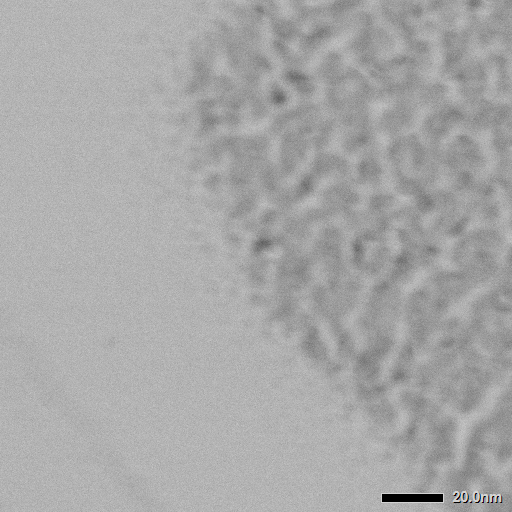
\includegraphics[width=\textwidth]{Gerüst/Abbildungen/STEM/STEM__20220817_1033_41_BF_ImagePanel3.png}
         \caption{BF}
         \label{astigBF}
     \end{subfigure}
     \hfill
     \begin{subfigure}[b]{0.49\textwidth}
         \centering
         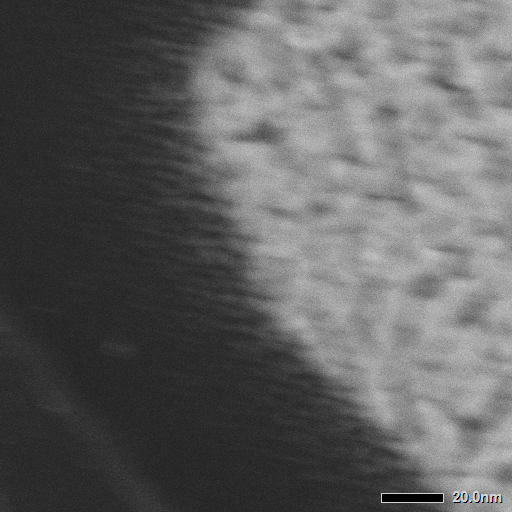
\includegraphics[width=\textwidth]{Gerüst/Abbildungen/STEM/STEM__20220817_1033_41_ADF1_ImagePanel1.png}
         \caption{HAADF}
         \label{astigDF}
     \end{subfigure}
        \caption{Unkorrigierte STEM Aufnahme von Au/Latex Probe}
        \label{STEMAstigmatismus}
\end{figure}

Zuerst wird mit dem Stigmator das Ronchigram so verzerrt das es symmetrisch ist und kleine Verzerrung in die X-/Y-Achse mehr erkennbar ist. Wenn man dann durch den Fokus wandert und die beiden Fokusse der Achsen an demselben Punkt sind, ist der Astigmatismus grob korrigiert. Später wird der restliche Fehler mit Hilfe der Mikroskop Software korrigiert.\\
Der Axiale Koma wird durch das verkippen des Strahles erreicht, dabei wird wieder durch den Fokus gefahren und so lange eingestellt bis das Bild symmetrisch durch den Fokus durchwandert. Die unendliche Vergrößerung ist dabei in der Mitte des Ronchigram. Diese Einstellungen wurden anschließend als Euzentrischer Fokus gespeichert. Das Korrigierte Ronchigram ist in der Aufnahme \cref{KorrRonchi} zu sehen, welches ausrechend verzerrungsfrei ist. Mit hilfe der Cs-Korrector software des mikroskops wurde der restliche Aberration gemessen und korrigiert. Die übrige Aberration nach deinem wiederholtem messen betrug: \(\zeta X: -0,2856 , Y: 0,4865 \).


\begin{figure}[H]
     \centering
  
         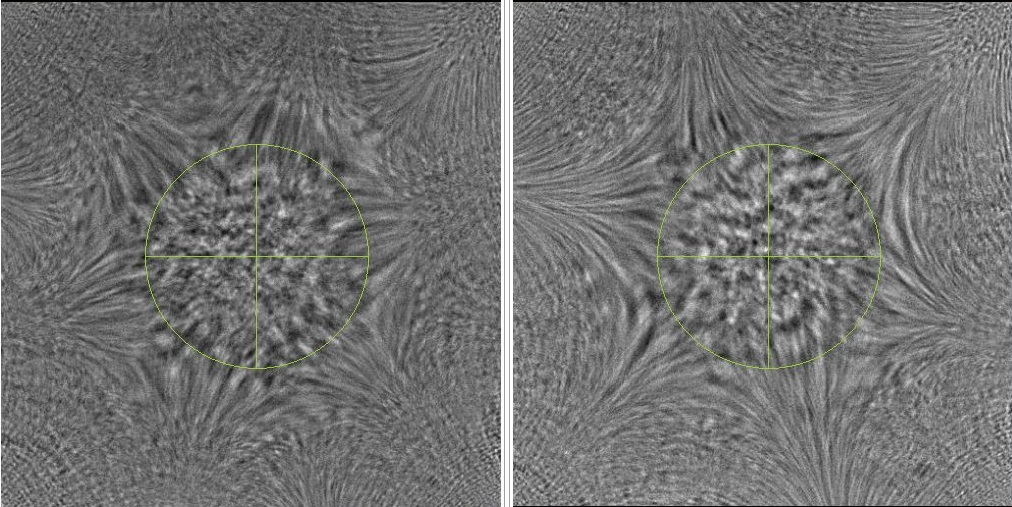
\includegraphics[width=\textwidth]{Gerüst/Abbildungen/STEM/corectors.jpg}
         \caption{Ronchigram im Über-/Underfokus nach der Aberration Korrektur}
         \label{KorrRonchi}

\end{figure}
Nach der Korrektur wurde eine Bildfehlerkorrigierte Aufnahmen im STEM Modus erstellt. Dabei wurde jedoch eine 30 µm \(Cl_2\) blende verwendet, die Abbildung \cref{STEMGold} zeigt die Goldcluster und Latex Kugeln. 
\begin{figure}
     \centering
     \begin{subfigure}[b]{0.3\textwidth}
         \centering
         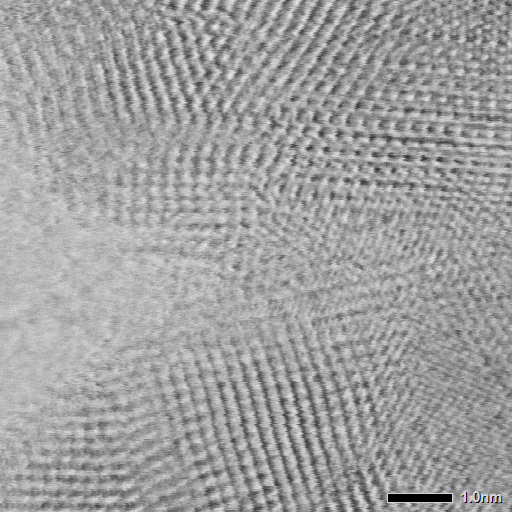
\includegraphics[width=\textwidth]{Gerüst/Abbildungen/STEM/STEM__20220817_1123_03_BF_ImagePanel3.png}
         \caption{BF}
         \label{STEMGoldBF}
     \end{subfigure}
     \hfill
     \begin{subfigure}[b]{0.3\textwidth}
         \centering
         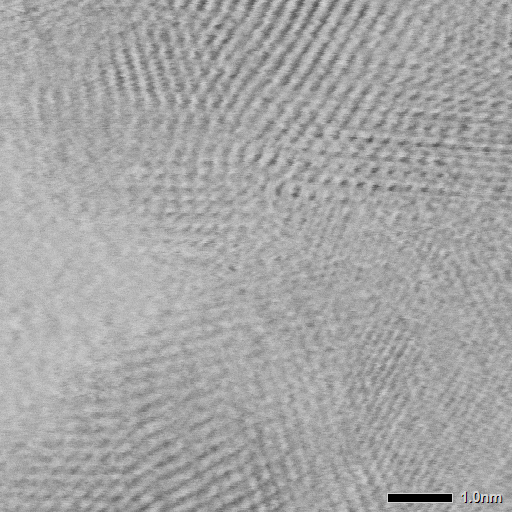
\includegraphics[width=\textwidth]{Gerüst/Abbildungen/STEM/STEM__20220817_1123_03_ABF_ImagePanel2.png}
         \caption{ADF}
         \label{STEMGoldADF}
     \end{subfigure}
     \hfill
     \begin{subfigure}[b]{0.3\textwidth}
         \centering
         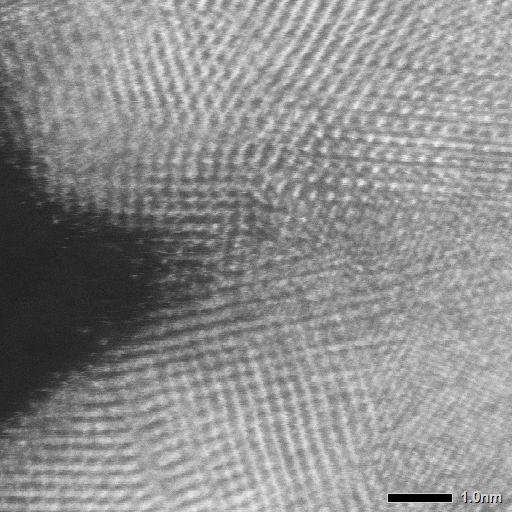
\includegraphics[width=\textwidth]{Gerüst/Abbildungen/STEM/STEM__20220817_1123_03_ADF1_ImagePanel1.png}
         \caption{HAADF}
         \label{STEMGoldHAADF}
     \end{subfigure}
        \caption{STEM Aufnahme der Standard Probe. Mit Gold Cluster in verschiedenen Orientierungen und Kohlefilm (Mitte Links)}
        \label{STEMGold}
\end{figure}
Es sind klar die reihenartige Anordnung der Goldatome in den Gold Cluster erkennbar, jedoch mit unterschiedliche orientierten Goldatome Domänen.\\
Der Kontrast unterscheidet sich erwartungsgemäß ebenfalls. So ist in \cref{STEMGoldHAADF} der Bereich des Kohlefilms dunkler abgebildet, was an der geringen Kernladungszahl des Kohlenstoffes liegt und Beugung an diesen Strukturen daher unter kleineren Winkeln stattfindet. Die Goldkluster hingegen mit hoher Kernladungszahl, bieten dagegen einen starken Kontrast.

\subsection{Eigene Probe}
Es wurde nun die Standard Gold/Latex Probe mit der selbst erstellten Probe eines Silizium Wafer getauscht, dieser Prozess ist zu einem großen Teil analog zum Proben Tauschen beim TITAN Mikroskop und die neue Einstellung und Korrektur ist analog zum vorher beschriebenen Prozess. Dieser Prozess ist unten nur in Stichpunkten zusammengefast:
\begin{itemize}
 \item Probenhalter Auswechseln.
 \item Check Vakuum
 \item Beam öffnen (Ventile)
 \item In „Low Mag“ Wechseln 
 \item Probe Verfahren, Loch mit Kante finden
 \item In STEM Modus wechseln
 \begin{itemize}
   \item Detektoren auswählen, ADF1, BF, HAADF
 \end{itemize}  
 \item Kamera Länge wechseln -> 8 cm
 \item Am Detektor dem Kontrast und Brightness neu einstellen
 \item Ins Rochigramm wechseln
 \item Kamera Länge auf 30 cm Wechseln
 \item CCD-Kamara Einfahren 
 \item Amorphen Bereich nahe der Kante suche
 \item Proben Höhe verstellen so das im Ronchigramm in Fokus ist.
 \item Vergrößerung 1M
 \item Astigmatismus korrigieren 
 \item Stigmatoren einstellen
 \begin{itemize}
   \item Inneren Bereich im Ronchigram möglichst groß 
 \end{itemize}  
 \item Astigmatismus Nachkorrigieren
 \item Probenstelle finden
 \item Im Substrat (Kristall) ist die Kikutchi Linien durch verkippen orientieren
 \item Probenhöhe anpassen
 \begin{itemize}
   \item Standard Fokus + Z Höhe
   \item Im maximalen Fokus
 \end{itemize}
 \item Blende Cl2 30 µm einfahren
 \begin{itemize}
  \item Blende zentrieren
 \end{itemize}
 \item Zurück zu den Sensoren Wechseln
 \item Kameralänge auf 6 cm
\end{itemize}

Es wurden von Vier stellen der Probe STEM aufnahmen erstellt, mit dem Ziel eine geeignete Stelle zu finden um die anschließende EDX Messungen durchzuführen.\\
Die erste Aufnahme Zeit eine Übersichtsaufnehme, es ist die Klebe stelle zwischen den beiden Wafer an welcher die Ionen Dünnung das Loch erstellt hat. In der Aufnahme sind beide Wafer Seiten zu sehen, es sind außerdem leiterbahnen, Transistoren und andere Mikrochip Elemente zu sehen, da sie einen sehr guten Kontrast im Bf und DF bieten. Es ist außerdem zu erkennen das die Probe an einigen Stellen sehr dünn ist da teilweise nur Teile der leiterbahnen noch frei im Vakuum stehen, wahren bei der Ionen Dünnung das umgebende Silizium entfernt wurde, \cref{STEMEigeneProbeUebersicht}
\begin{figure}[H]
     \centering
     \begin{subfigure}[b]{0.49\textwidth}
         \centering
         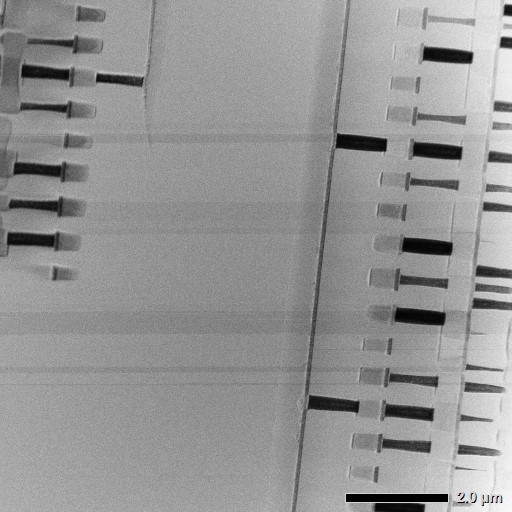
\includegraphics[width=\textwidth]{Gerüst/Abbildungen/STEM/EigeneProbeBFUebersicht.jpeg}
         \caption{BF}
         \label{UeberBF}
     \end{subfigure}
     \hfill
     \begin{subfigure}[b]{0.49\textwidth}
         \centering
         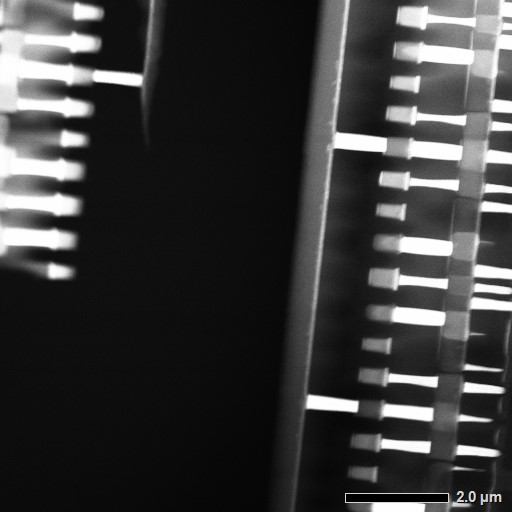
\includegraphics[width=\textwidth]{Gerüst/Abbildungen/STEM/EigeneProbeHAADFUebersicht.jpeg}
         \caption{HAADF}
         \label{UeberDF}
     \end{subfigure}
        \caption{STEM Übersichtsaufnahme der eigenen Probe}
        \label{STEMEigeneProbeUebersicht}
\end{figure}
In der zweiten Aufnahme \cref{Pos1} ist eine leiterbahn zu sehen, mit denselben Bauteilen wie in der Übersicht Aufnahme außerdem ist ein größerer Teil des Silizium Volumen abgebildet, dort sind im BF mehrere Biegekonturen zu sehen.\\
In der dritten Aufnahme ist die leiterbahn mit unterschiedlichen Halbleiter Elementen zusehen. Hier wurde eine Größere Vergrößerung verwendet, diese Aufnahme ist von Oberen linken Rand des Loches, \cref{Pos2}.\\
Die vierte Aufnahme ist vom derselben leiterbahn am unter linken Ende des Lochs.  Die Probe ist hier etwas dicker als an der oberen Seite des Lochs, \cref{Pos3}.\\
Das fünfte Bild wurde von der rechten unteren Seite des Lochs erstellt, die Probe ist hier ziemlich dünn und weist eine der uniforme dicke auf, \cref{Pos4}.\\ 
Dieser Stelle der Probe wird anschließend für die EDX Messungen verwendet. Die Durchstahlbarkeit ist an dieser stell ist sehr gut, dies ist im BF Image gut erkennbar da die gesamte Probe hell beleuchtet wird, vom Vakuum bis zur dickste Stelle weit vom lock entfernt.\\
Die ADF und HAADF Bilder (\cref{Pos4ADF} und \cref{Pos4HAADF}) liefert auch einen sehr guten Kontrast welches auf die Kristallstruktur und gut unterscheidbaren Z werte deutet.  Es ist zusätzlich zu erkennen das die an der dünneren stellen der Probe i.e. nahe des loch, die Aufnahme heller ist. Also mehr gestreute Elektronen in der Lage sind dem Volumen zu entkommen und gemessen werden. Außerdem ist eine Beugungskontur nahe der Kante erkennbar.



\begin{figure}[H]
     \centering
     \begin{subfigure}[b]{0.4\textwidth}
         \centering
         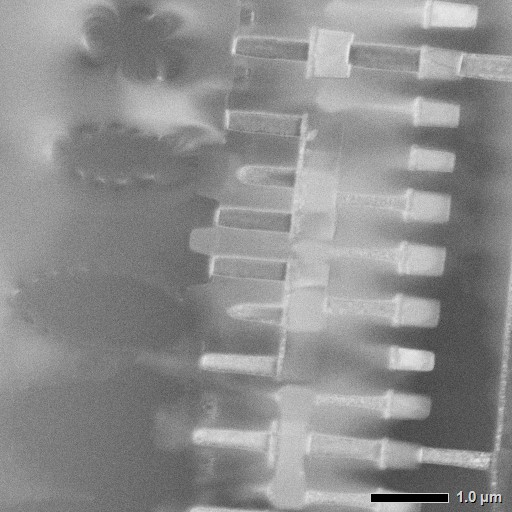
\includegraphics[width=\textwidth]{Gerüst/Abbildungen/STEM/EigeneProbeBFPos1.jpeg}
         \caption{Position 1}
         \label{Pos1}
     \end{subfigure}
     \hfill
     \begin{subfigure}[b]{0.4\textwidth}
         \centering
         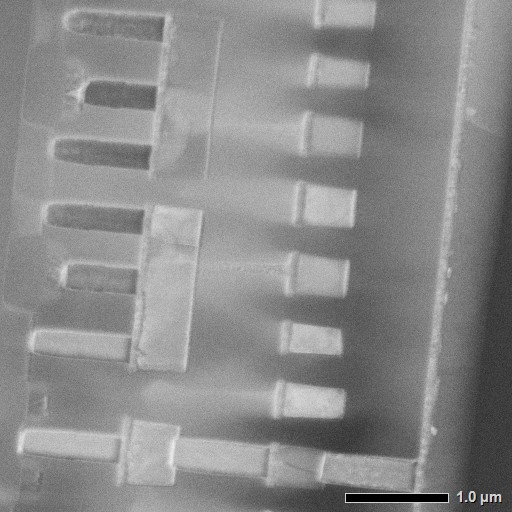
\includegraphics[width=\textwidth]{Gerüst/Abbildungen/STEM/EigeneProbeBFPos2.jpeg}
         \caption{Position 2}
         \label{Pos2}
     \end{subfigure}
      
 %\vspace{}

 \centering
     \begin{subfigure}[b]{0.4\textwidth}
         \centering
         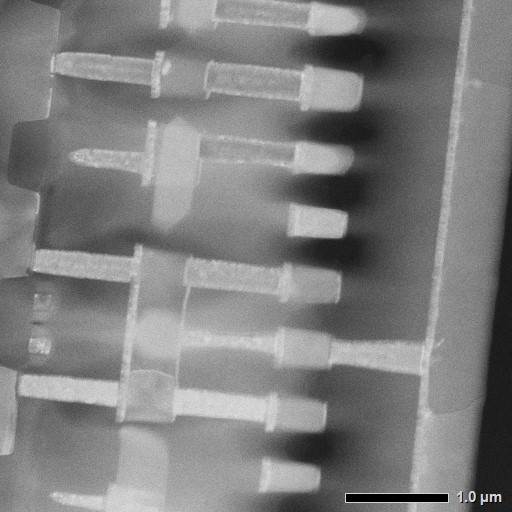
\includegraphics[width=\textwidth]{Gerüst/Abbildungen/STEM/EigeneProbeBFPos3.jpeg}
         \caption{Position 3}
         \label{Pos3}
     \end{subfigure}
     \hfill
     \begin{subfigure}[b]{0.4\textwidth}
         \centering
         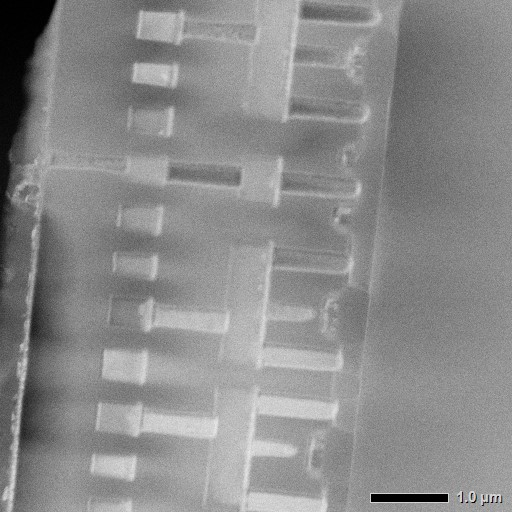
\includegraphics[width=\textwidth]{Gerüst/Abbildungen/STEM/EigeneProbeBFPos4.jpeg}
         \caption{Position 4}
         \label{Pos4}
     \end{subfigure}
     
      \centering
     \begin{subfigure}[b]{0.4\textwidth}
         \centering
         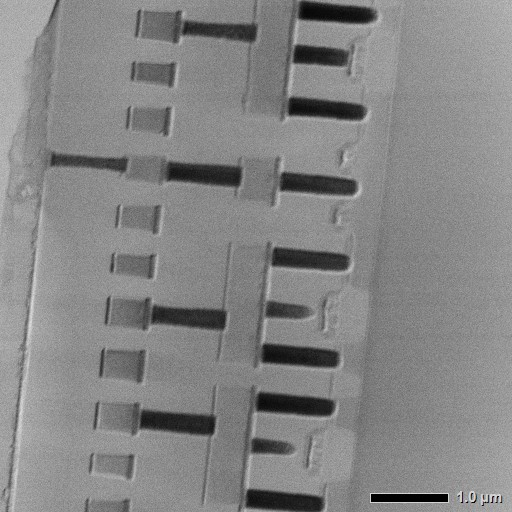
\includegraphics[width=\textwidth]{Gerüst/Abbildungen/STEM/EigeneProbeBFPos4ADF.jpeg}
         \caption{Position 4, ADF}
         \label{Pos4ADF}
     \end{subfigure}
     \hfill
     \begin{subfigure}[b]{0.4\textwidth}
         \centering
         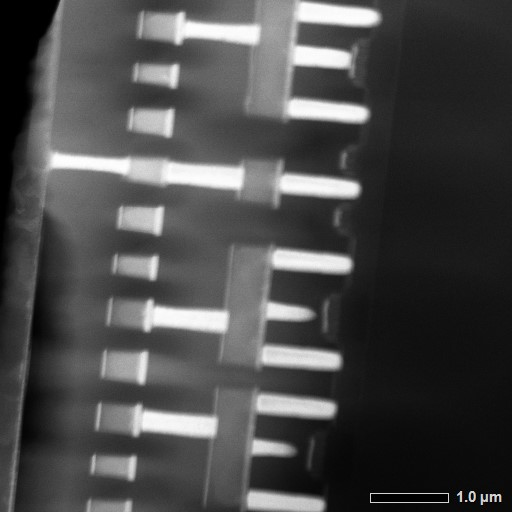
\includegraphics[width=\textwidth]{Gerüst/Abbildungen/STEM/EigeneProbeBFPos4HAADF.jpeg}
         \caption{Position 4, HAADF}
         \label{Pos4HAADF}
     \end{subfigure}
     
     \caption{BF aufnahmen an Vier Verschiedenen Positionen an der eigenen Probe, ADF und HAADF Aufnahmen an der Position 4}
        \label{EigeneProbeBFPositionen}
 
\end{figure}

\section{STEM-EDX}
\subsection{EDX (energy dispersive X-ray)}
Beim EDX wird die Charakteristische Röntgenstrahlung gemessen die bei der Anregung des Atoms durch den Elektronenstrahl entsteht. Die Charakteristik Röntgenstrahlung entsteht, wenn ein hoch energetisches Anregungselektron ein innerschalen Elektron herausschlägt. Anschließend wird das entstandene Elektronenloch durch ein höherschaliges Elektron gefühlt, dabei wird ein hochenergetisches röntgen Photon freigesetzt. Dieses Photon entspricht der Energie Differenz der involvierten Schalen und ist damit charakteristisch für das Atom und die Energieschalen, so das ein Element eindeutig identifizierbar ist.\\
Bei der Anregung durch hoch energetische Elektronen wird zusätzlich Bremsstrahlung freigesetzt welche allerdings nicht charakteristisch für das Element ist. \\
In EDX Messungen werden zusätzlich charakteristische Strahlung von dem umgebenden Mikroskop: Probenhalter, Linse, Elektronenquelle etc. durch sekundäre Prozesse freigesetzt. Diese Störsignale werden auch gemessen und müssen in der Auswertung berücksichtigt werden.
Ein EDX Detektor wird heutzutage meistens mit einem SDD (Silicon Drift Detektor) betrieben, dieser ist aus einem Halbleiter gefertigt welcher die Energie eines Röntgenphotons misst indem er die Ionisation im Halbleiter durch das Photon misst. Dabei sind P gedopte Übergänge auf der oberflache des Detektors angebracht, wenn die Strahlung im Volumen des Detektors ionisiert wird driften anschließend die freigesetzten Elektronen zu einer Anode. Die dabei entstehende Ladung an der Anode kann anschließen gemessen und ausgewertet werden um die Energie des Photons zu bestimmen. Es muss jedoch darauf geachtet werden das die Intensität auf dem Detektor nicht zu groß ist da zwei Photonen die zeitlich sehr dicht beieinander den Detektor treffen zusammen gemessen werden können und sich dadurch die gemessene Energie der beiden Photonen addieren. (PileUp-Effekte).\\
Mit Hilfe des EDX kann eine Hoch aufgelöste elementare Verteilung in der Probe erstellt werden.

\subsection{STEM-EDX Versuch}
In diesem Teil war das Ziel ein EDX Mapping von dem zuvor ausgewählten Proben Region zu erstellen. Da wie zuvor erwähnt das Mikroskop selbst einen relevante Background Röntgenstrahlung produziert, muss diese in der Analyse berücksichtigt werden. Dafür wurde zuerst eine Background Aufnahme erstellt in der die Probe aus dem Elektronen strahl entfernt wird und ausschließlich Vakuum gemessen wird. In Aufnahme \cref{EDXSpecBG} ist das gemessen Spektrum zu sehen. In diesem Spektrum konnten die Peaks vom:  C, O, Fe, N Al, Au, Mo, Ti, W, Co und Cu gemessen werden. Einige dieser Peaks sind mit Kontamination zu erklären, z.B. C, N und O. Andere sind von Bauteilen des Mikroskops, wie Linsenpolschuhe, Magnetspulen, etc., diese Peaks sind von: Fe, Al, Ti, Co und Cu. Von Strahlenschutz Beschichtungen sind zum Beispiel die Ag Peaks. Die W Peaks sind durch Kontaminirung FETs zu erklären, sogenante Tungsten-Plays.

\begin{figure}[H]
     \centering
     \begin{subfigure}[b]{0.49\textwidth}
         \centering
         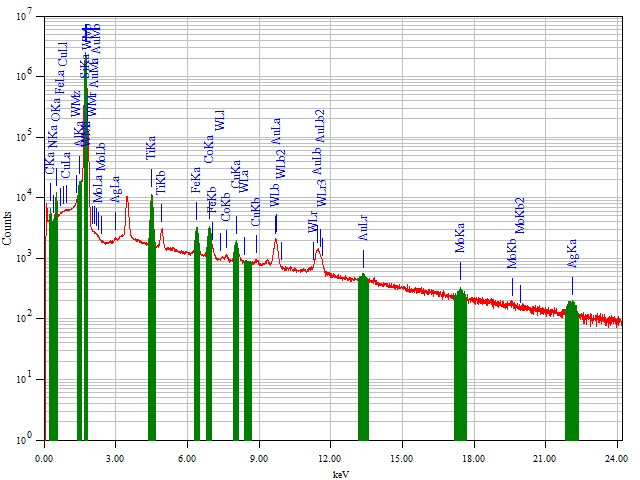
\includegraphics[width=\textwidth]{Gerüst/Abbildungen/EDX/SpektrumBackground.jpg}
         \caption{Background}
         \label{EDXSpecBG}
     \end{subfigure}
     \hfill
     \begin{subfigure}[b]{0.49\textwidth}
         \centering
         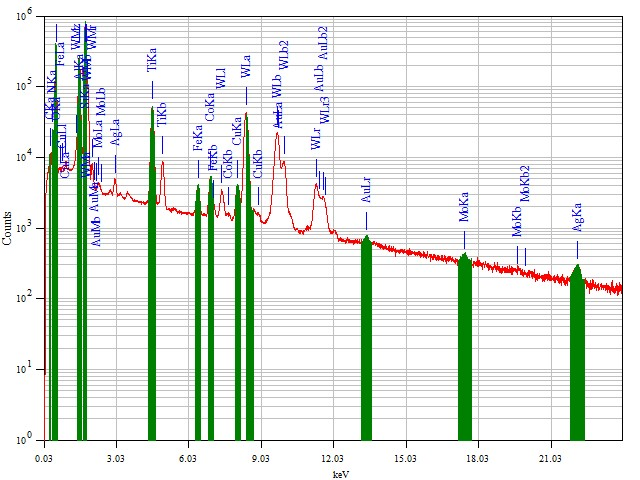
\includegraphics[width=\textwidth]{Gerüst/Abbildungen/EDX/Spektrum.jpg}
         \caption{Probe}
         \label{EDXSpecProb}
     \end{subfigure}
        \caption{EDX Spektrum Aufnahmen der Hintergrunds Strahlung und der der Eigenen Si Probe}
        \label{EDX}
\end{figure}

Anschließend wurde die Probe wieder an die vorherige Position eingefahren und eine EDX-Aufnahme erstellt. Das Resultierende Spektrum ist in Abbildung \cref{EDXSpecProb} zu sehen. In diesem sind die N, F, O, Al und Co Starker ausgeprägt und zusätzlich ist die Si Peaks abgebildet.\\
Der Kohlenstoff auf der Probe ist mit hoher Wahrscheinlichkeit durch Kontamination entstanden. Da es ziemlich gleichmäßig auf der gesamten Probe erkennbar ist, außerdem ist er starker in dem hohen Kontrast Bereichen abgebildet, in den vor allem Metalle gemessen werden wie Al, W und Ti. Die Vermutung liegt nahe das dieser Starke C Kontrast durch Bremsstrahlung und sekundäre Effekte erzeugt wird welche unterstutzt wird mit der Kohlenstoff Abbildung bei der die Bremsstrahlung abgezogen wurde. Dort ist die Verteilung über die gesamte Probe sehr viel homogener, \cref{EDXC}.

\begin{figure}[H]
     \centering
     \begin{subfigure}[b]{0.49\textwidth}
         \centering
         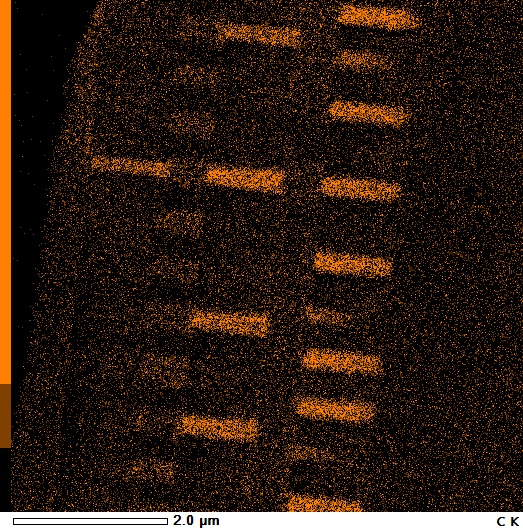
\includegraphics[width=\textwidth]{Gerüst/Abbildungen/EDX/OhneSystemPeaks C K.jpg}
         \caption{Mit Bremsstrahlung}
         \label{EDXCmBS}
     \end{subfigure}
     \hfill
     \begin{subfigure}[b]{0.49\textwidth}
         \centering
         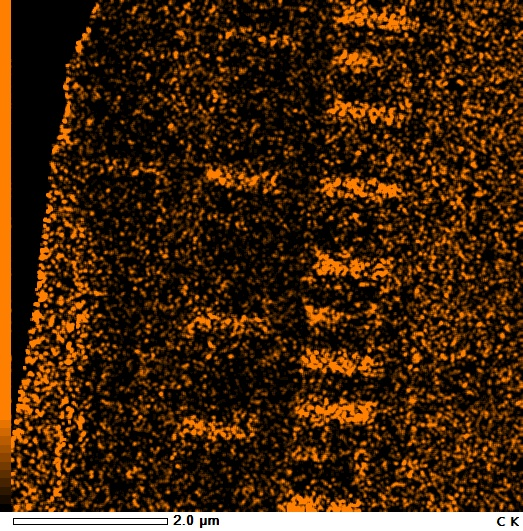
\includegraphics[width=\textwidth]{Gerüst/Abbildungen/EDX/QuantAnalyse_ohneBremsstrahlung C K.jpg}
         \caption{Ohne Bremsstrahlung}
         \label{EDXCoBS}
     \end{subfigure}
        \caption{EDX Map von Kohlenstoff mit und ohne Bremsstrahlung}
        \label{EDXC}
\end{figure}

Sauerstoff ist auf der Probe auch recht homogen verteil, jedoch sind sehr klare Strukturen von Sauerstoff armen/leeren Regionen zu sehen, \cref{EDXO}. Die Sauerstoff verarmten Zonen sind vor allem an Mikrochip Elementen die Metalle aufweisen wie Al, Ti enthalten, diese sind wahrscheinlich die leiterbahnen und Transistoren. Außerdem ist im Volumen des Chips (hinter der letzten leiterbahn, rechts), kein Sauerstoff vorhanden. In der Si Aufnahme \cref{EDXSi} ist auch zu erkennen, dass das eine reine Silizium Region ist, wahrscheinlich der ursprüngliche Wafer aus einem perfekten Silizium Chip bevor er weiterverarbeitet wurde. Der Sauerstoff ist möglicherweise auf die Probe bei der Verbreitung des Wafers gekommen, vielleicht bei lithographischen Prozessen, ob es eine Verunreinigung oder systemrelevant ist kann nicht beantwortet werden.

\begin{figure}
     \centering
     \begin{subfigure}[b]{0.3\textwidth}
         \centering
         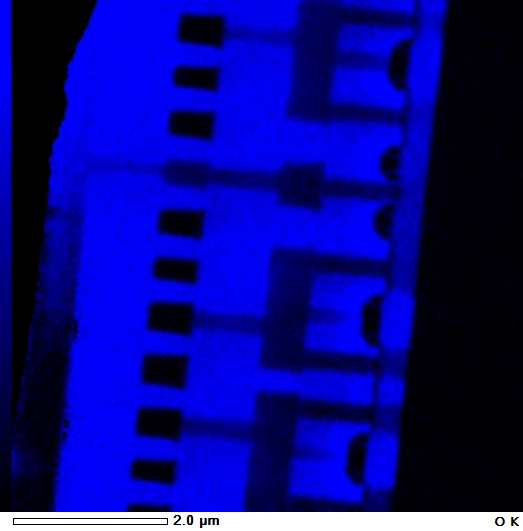
\includegraphics[width=\textwidth]{Gerüst/Abbildungen/EDX/QuantAnalyse_ohneBremsstrahlung O K.jpg}
         \caption{O}
         \label{EDXO}
     \end{subfigure}
     \hfill
     \begin{subfigure}[b]{0.3\textwidth}
         \centering
         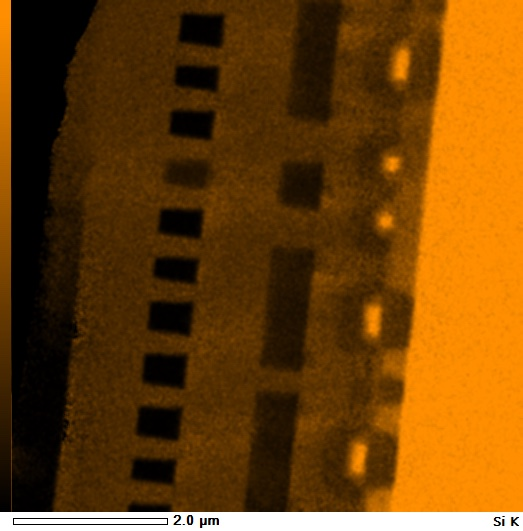
\includegraphics[width=\textwidth]{Gerüst/Abbildungen/EDX/QuantAnalyse_ohneBremsstrahlung Si K.jpg}
         \caption{Si}
         \label{EDXSi}
     \end{subfigure}
     \hfill
     \begin{subfigure}[b]{0.3\textwidth}
         \centering
         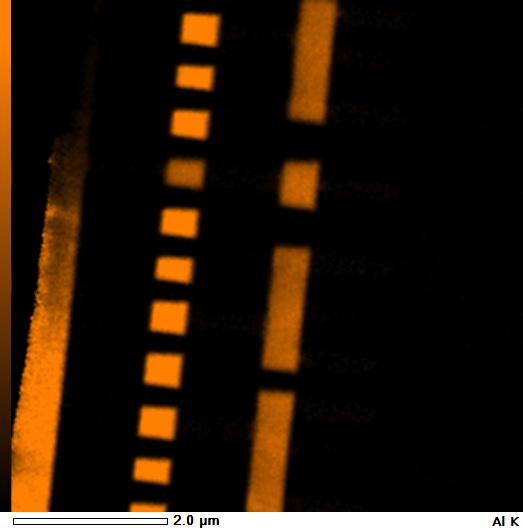
\includegraphics[width=\textwidth]{Gerüst/Abbildungen/EDX/QuantAnalyse_ohneBremsstrahlung Al K.jpg}
         \caption{Al}
         \label{EDXAl}
     \end{subfigure}
        \caption{EDX Maps von Sauerstoff, Silikat und Aluminium, ohne Bremsstrahlung}
        \label{EDXCSiAl}
\end{figure}

Das Aluminium auf der Probe ist ausschließlich in den leiterbahnen verwendet worden, es hat einen sehr starken Kontrast und diese Regionen werden in den anderen EDX Element Mapps leer (dunkel) dargestellt, \cref{EDXAl}.


\begin{figure}[H]
     \centering
     \begin{subfigure}[b]{0.49\textwidth}
         \centering
         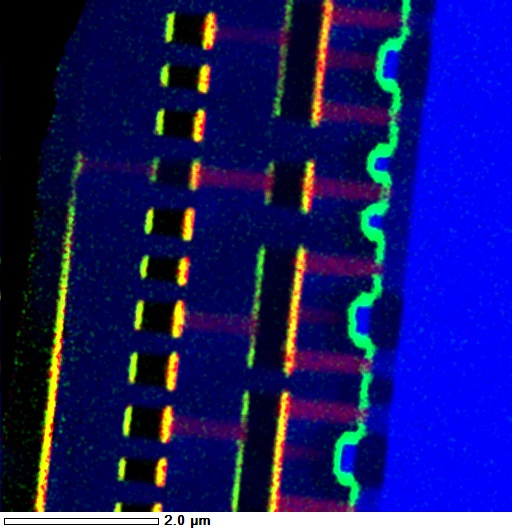
\includegraphics[width=\textwidth]{Gerüst/Abbildungen/EDX/Overlay(Si_N_Ti) OVERLAY.jpg}
         \caption{Si:B, N:G, Ti:R}
         \label{Overlay}
     \end{subfigure}
     \hfill
     \begin{subfigure}[b]{0.49\textwidth}
         \centering
         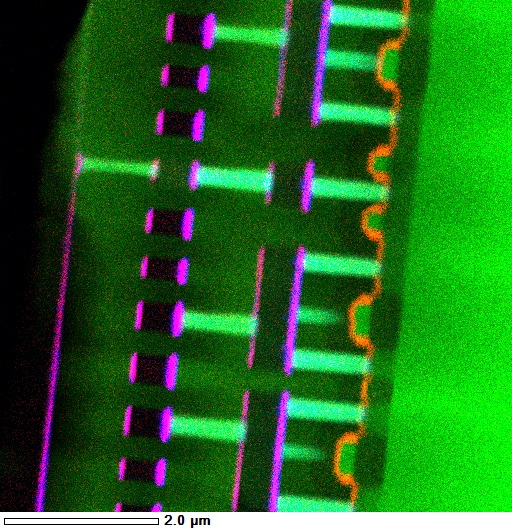
\includegraphics[width=\textwidth]{Gerüst/Abbildungen/EDX/Overlay(Ti_Si_N) OVERLAY.jpg}
         \caption{Ti:B Si:G, N:R}
         \label{Overlay2}
     \end{subfigure}
        \caption{EDX Map Overlay der Eigen Probe von Titan, Silikat und Stickstoff}
        \label{EDXOverlay}
\end{figure}

Die besonderes Spannenden Mapps sind die der Ti, Si und N, um diese besser zu verstehen und zuzuordnen sind sie am besten in den beiden Overlay aufnahmen \cref{EDXOverlay} dargestellt, hier kann man einen sehr guten N Kontrast am der rechten Seiter des linken Al leiterband sehen, und an den Rändern der anderen Leitungsbahnen. Was das N an diesen Stellen bewirkt kann nicht gesagt werden aber es scheint für den Übergang zwischen Si und Al relevant zu sein. Das Titan scheint eine Rolle für das dopen des Si zu spielen, es ist an den Al Leiterband Übergängen zu sehen, aber auch an eigenen leiterbahnen die die AL bahnen verbinden. Es ist zusätzlich ein leichter Kontrast im Si an der linken Al leiterbahn zu sehen, es wird vermutet das diese die Transistoren sind, aber eine Bestimmung ist aus Mengel an Wissen über Halbleiter und Mikrochips nicht möglich.

